\title{%
  Intro till en kurs i programmeringsteknik
}
\author{Daniel Bosk}
\institute{%
  KTH EECS
}

\mode<article>{\maketitle}
\mode<presentation>{%
  \begin{frame}
    \maketitle
  \end{frame}
}

\mode*

\begin{abstract}
  % What's the problem?
% Why is it a problem? Research gap left by other approaches?
% Why is it important? Why care?
% What's the approach? How to solve the problem?
% What's the findings? How was it evaluated, what are the results, limitations, 
% what remains to be done?

% XXX Summary
\emph{Summary:}
\dots

% XXX Motivation and intended learning outcomes
\emph{Intended learning outcomes:}
\dots

% XXX Prerequisites
\emph{Prerequisites:}
\dots

% XXX Reading material
\emph{Reading:}
\dots

\end{abstract}


\section{Vilka är vi?}

\subsection{Lärare}

\begin{frame}
  \begin{block}{Kursansvarig lärare}
    \begin{itemize}
      \item Namn: Daniel Bosk
      \item Lärarutbildad i matematik och datateknik (CL, 2006--2011) vid KTH 
        och Stockholms universitet (f.d. Lärarhögskolan)
      \item Forskarutbildad i datalogi (2014--2020) vid KTH
      \item Undervisat på universitetsnivå sedan 2011.
      \item Fokus på e-lärande och distansundervisning.
    \end{itemize}
  \end{block}
\end{frame}

\begin{frame}
  \begin{center}
    Övningsledare
  \end{center}
\end{frame}

\begin{frame}
  \begin{center}
    Labbhandledare
  \end{center}
\end{frame}

\subsection{Studenter}

\begin{frame}
  \begin{exercise}[Vad ha ni för intressen?]
    \begin{itemize}
      \item Gå till \url{menti.com} och ange koden 78 28 93 5.
    \end{itemize}
  \end{exercise}
\end{frame}

\begin{frame}
  \begin{exercise}[Vilka är ni?]
    \begin{itemize}
      \item Break-out rooms: tre personer i varje.
      \item Var kommer ni från?
      \item Varför kom ni hit?
      \item Var är ni på väg?
    \end{itemize}
  \end{exercise}
\end{frame}


\section{Varför ska ni läsa programmering?}

\begin{frame}
  \begin{center}
    Äldre motiverar varför för yngre.
  \end{center}
\end{frame}


\section{Om kursen}

\subsection{Vad ska ni få ut?}

\begin{frame}
  \begin{block}<+>{Färdigheter}
    \begin{itemize}
      \item Algoritmiskt tänkande
      \item Problemlösningsförmåga
    \end{itemize}
  \end{block}

  \begin{block}<+>{Kunskaper}
    \begin{itemize}
      \item Terminologi
      \item Mental modell av datorsystem
    \end{itemize}
  \end{block}

  \begin{block}<+>{Verktyg}
    \begin{itemize}
      \item Python
      \item Matlab
    \end{itemize}
  \end{block}
\end{frame}

\subsection{Hur ska ni få ut detta?}

\begin{frame}
  \begin{block}{Moduler}
    \begin{enumerate}
      \item Förberedelse
      \item Föreläsning
      \item Laboration
      \item Föreläsning
      \item Övning
    \end{enumerate}
  \end{block}

  \pause

  \begin{block}{Projekt}
    \begin{itemize}
      \item Större uppgift.
      \item Andra halvan av kursen.
    \end{itemize}
  \end{block}
\end{frame}

\begin{frame}
  \begin{block}{Förberedelse}
    \begin{itemize}
      \item Egna studier: OLI och FeedbackFruits.
      \item Interaktionen bra för lärande.
    \end{itemize}
  \end{block}

  \pause
  
  \begin{block}{\enquote{Föreläsningar}}
    \begin{itemize}
      \item Ger en översiktlig genomgång.
      \item Fokuserar på de viktigaste delarna.
      \item Får information från interaktionen under era förberedelser.
      \item Praktisk problemlösning för er!
    \end{itemize}
  \end{block}
\end{frame}

\begin{frame}
  \begin{block}{Laborationer}
    \begin{itemize}
      \item Driver ert lärande framåt.
      \item Lärande är socialt, arbeta i grupper om två.
    \end{itemize}
  \end{block}

  \pause

  \begin{remark}
    \begin{itemize}
      \item Skapa studiegrupper!
    \end{itemize}
  \end{remark}

  \pause

  \begin{block}{Övningar}
    \begin{itemize}
      \item Interaktiva tillfällen för lärande.
      \item Bygger vidare på laborationerna.
    \end{itemize}
  \end{block}
\end{frame}

\begin{frame}
  \begin{exercise}[Hur studerar ni?]
    \begin{itemize}
      \item Break-out rooms: tre nya personer i varje.
      \item Hur har du studerat bäst hittills? Vad är din studieteknik?
    \end{itemize}
  \end{exercise}
\end{frame}

\subsection{Hur kollar vi att ni kan?}

\begin{frame}
  \begin{block}<+>{Laborationer (LAB1, 1.5 hp)}
    \begin{itemize}
      \item Lämnas in i Canvas.
      \item Måste även delta i övningen.
      \item \emph{Man får misslyckas}, bara att fixa och lämna in igen!
      \item Första halvan av kursen.
    \end{itemize}
  \end{block}

  \pause

  \begin{block}<+>{Datorprov (LAB2, 1.5 hp)}
    \begin{itemize}
      \item Testar era kunskaper efter att vi täckt allt material.
      \item Mitten av kursen.
      \item Ges en gång i månaden så länge det finns behov.
    \end{itemize}
  \end{block}
\end{frame}

\begin{frame}
  \begin{block}{P-uppgift (LAB3, 3.0 hp)}
    \begin{itemize}
      \item Testar era färdigheter.
      \item Låter er utvecklas djupare.
      \item Andra halvan av kursen.
      \item Betyget baseras på denna.
    \end{itemize}
  \end{block}
\end{frame}

\begin{frame}
  \begin{block}{Matlablaborationen (MAT1, 1.5 hp)}
    \begin{itemize}
      \item Examinerar Matlabfärdigheter
      \item Innan P-uppgiften drar igång.
    \end{itemize}
  \end{block}
\end{frame}


\section{Disciplinära förseelser}

\mode<all>{\begin{frame}
  
\includegraphics[width=\columnwidth]{fig/SverigesRikesLag.png}
\end{frame}

\begin{frame}
  \begin{block}{10 kap. Högskoleförordningen (1993:100)\nocite{SFS1993:100}}
    \textbf{Allmänna bestämmelser}

    \vspace{0.5em}
    1 §   Disciplinära åtgärder får vidtas mot studenter som
    \begin{enumerate}
      \item med otillåtna hjälpmedel eller på annat sätt försöker vilseleda vid 
        prov eller när en studieprestation annars ska bedömas,
      \item stör eller hindrar undervisning, prov eller annan verksamhet inom 
        ramen för utbildningen vid högskolan,
      \item stör verksamheten vid högskolans bibliotek eller annan särskild 
        inrättning inom högskolan, eller
      \item utsätter en annan student eller en arbetstagare vid högskolan för 
        sådana trakasserier eller sexuella trakasserier som avses i 1 kap. 4 § 
        diskrimineringslagen (2008:567).
    \end{enumerate}
  \end{block}
\end{frame}

\begin{frame}
  \begin{block}{10 kap. Högskoleförordningen (1993:100)\nocite{SFS1993:100}, 
    forts.}
    \textbf{Disciplinära åtgärder}

    \vspace{0.5em}
    2 § De disciplinära åtgärderna är varning och avstängning.

    \vspace{0.5em}
    Ett beslut om avstängning innebär att studenten inte får delta i 
    undervisning, prov eller annan verksamhet inom ramen för utbildningen vid 
    högskolan. Beslutet skall avse en eller flera perioder, dock sammanlagt 
    högst sex månader.

    \vspace{0.5em}
    Ett beslut om avstängning får också begränsas till att avse tillträde till 
    vissa lokaler inom högskolan.
  \end{block}
\end{frame}

\begin{frame}
  \begin{block}{10 kap. Högskoleförordningen (1993:100)\nocite{SFS1993:100}, 
    forts.}
    \textbf{Disciplinnämnden}

    \vspace{0.5em}
    3 § Ärenden om disciplinära åtgärder skall, om inte annat följer av 9 §, 
      handläggas av en disciplinnämnd. En sådan nämnd skall finnas vid varje 
      högskola.

    \vspace{0.5em}
    4 § Disciplinnämnden skall bestå av rektor som ordförande, en lagfaren 
      ledamot som skall vara eller ha varit ordinarie domare och en företrädare 
      för lärarna vid högskolan. Studenterna vid högskolan har rätt att vara 
      representerade i nämnden med två ledamöter. Förordning (1998:1003).
  \end{block}
\end{frame}

\begin{frame}
  \begin{block}{10 kap. Högskoleförordningen (1993:100)\nocite{SFS1993:100}, 
    forts.}
    13 §   När ett beslut om avstängning har fattats, skall underrättelser om 
       detta genast tillställas Centrala studiestödsnämnden och de organ inom 
       högskolan som berörs.
  \end{block}
\end{frame}

\begin{frame}
  
\includegraphics[width=\columnwidth]{fig/uu-domstol.png}
\end{frame}

\begin{frame}
  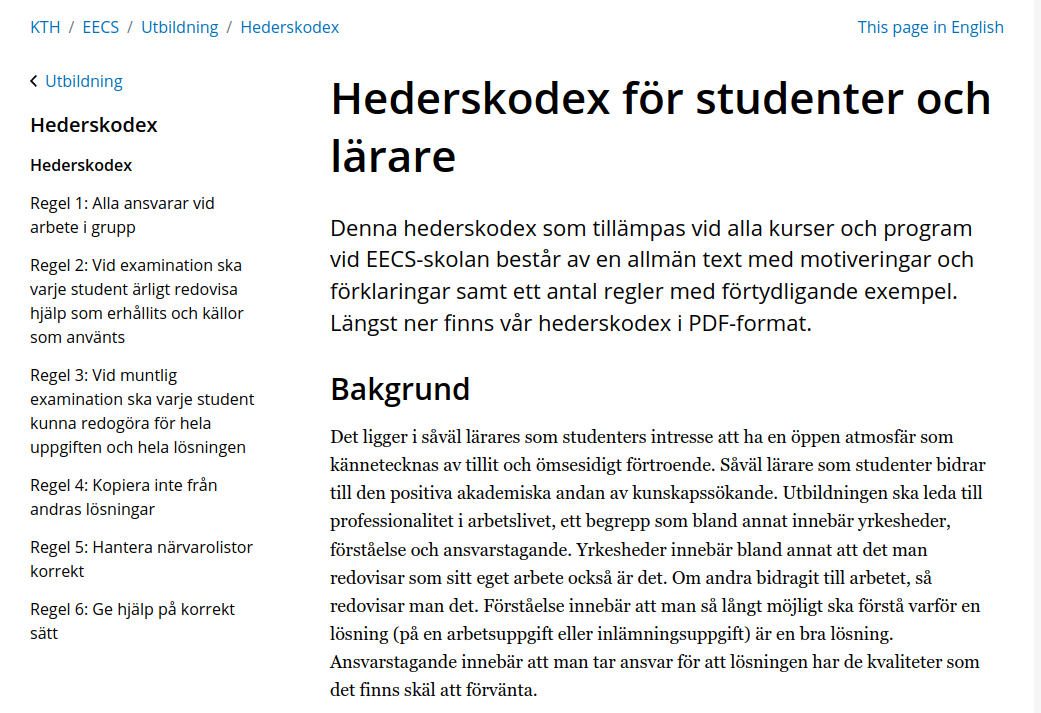
\includegraphics[width=\columnwidth]{fig/hederskodex.png}
\end{frame}
}



\section{Kursens material}

\begin{frame}
  \begin{figure}
    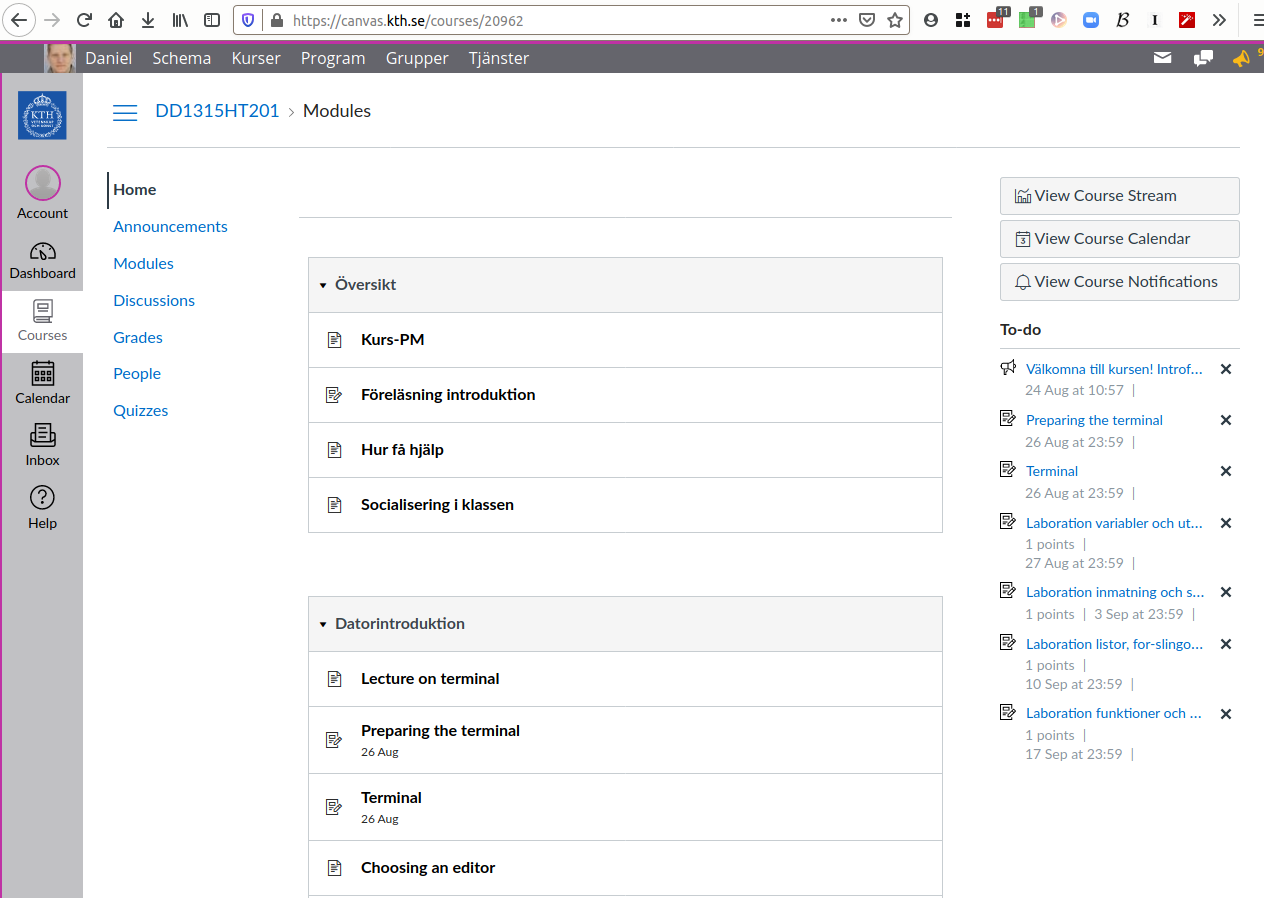
\includegraphics[height=0.8\textheight]{canvas.png}
    \caption{Demo av Canvas}
  \end{figure}
\end{frame}

